% Created by tikzDevice version 0.11 on 2018-04-06 11:09:08
% !TEX encoding = UTF-8 Unicode
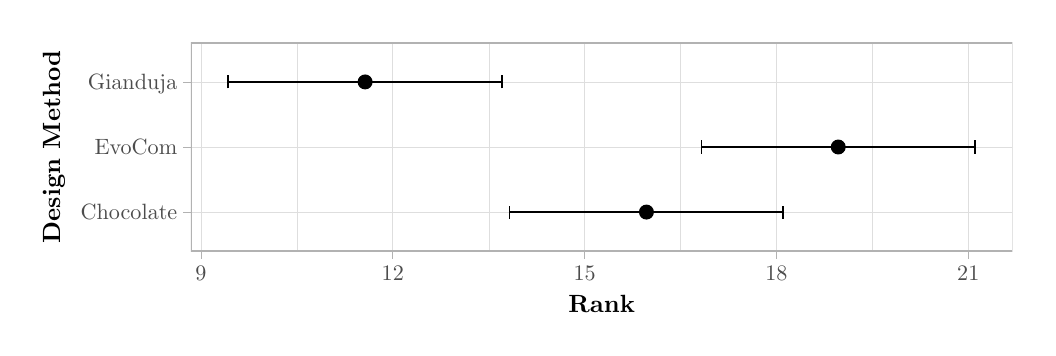
\begin{tikzpicture}[x=1pt,y=1pt]
\definecolor{fillColor}{RGB}{255,255,255}
\path[use as bounding box,fill=fillColor,fill opacity=0.00] (0,0) rectangle (361.35,108.41);
\begin{scope}
\path[clip] (  0.00,  0.00) rectangle (361.35,108.41);
\definecolor{drawColor}{RGB}{255,255,255}
\definecolor{fillColor}{RGB}{255,255,255}

\path[draw=drawColor,line width= 0.6pt,line join=round,line cap=round,fill=fillColor] (  0.00,  0.00) rectangle (361.35,108.41);
\end{scope}
\begin{scope}
\path[clip] ( 58.99, 27.67) rectangle (355.85,102.91);
\definecolor{fillColor}{RGB}{255,255,255}

\path[fill=fillColor] ( 58.99, 27.67) rectangle (355.85,102.91);
\definecolor{drawColor}{gray}{0.87}

\path[draw=drawColor,line width= 0.1pt,line join=round] ( 97.29, 27.67) --
	( 97.29,102.91);

\path[draw=drawColor,line width= 0.1pt,line join=round] (166.60, 27.67) --
	(166.60,102.91);

\path[draw=drawColor,line width= 0.1pt,line join=round] (235.91, 27.67) --
	(235.91,102.91);

\path[draw=drawColor,line width= 0.1pt,line join=round] (305.22, 27.67) --
	(305.22,102.91);

\path[draw=drawColor,line width= 0.3pt,line join=round] ( 58.99, 41.78) --
	(355.85, 41.78);

\path[draw=drawColor,line width= 0.3pt,line join=round] ( 58.99, 65.29) --
	(355.85, 65.29);

\path[draw=drawColor,line width= 0.3pt,line join=round] ( 58.99, 88.80) --
	(355.85, 88.80);

\path[draw=drawColor,line width= 0.3pt,line join=round] ( 62.63, 27.67) --
	( 62.63,102.91);

\path[draw=drawColor,line width= 0.3pt,line join=round] (131.94, 27.67) --
	(131.94,102.91);

\path[draw=drawColor,line width= 0.3pt,line join=round] (201.26, 27.67) --
	(201.26,102.91);

\path[draw=drawColor,line width= 0.3pt,line join=round] (270.57, 27.67) --
	(270.57,102.91);

\path[draw=drawColor,line width= 0.3pt,line join=round] (339.88, 27.67) --
	(339.88,102.91);
\definecolor{drawColor}{RGB}{0,0,0}
\definecolor{fillColor}{RGB}{0,0,0}

\path[draw=drawColor,line width= 0.4pt,line join=round,line cap=round,fill=fillColor] (223.59, 41.78) circle (  2.50);

\path[draw=drawColor,line width= 0.4pt,line join=round,line cap=round,fill=fillColor] (292.90, 65.29) circle (  2.50);

\path[draw=drawColor,line width= 0.4pt,line join=round,line cap=round,fill=fillColor] (121.93, 88.80) circle (  2.50);

\path[draw=drawColor,line width= 0.6pt,line join=round] (273.04, 39.43) --
	(273.04, 44.13);

\path[draw=drawColor,line width= 0.6pt,line join=round] (273.04, 41.78) --
	(174.14, 41.78);

\path[draw=drawColor,line width= 0.6pt,line join=round] (174.14, 39.43) --
	(174.14, 44.13);

\path[draw=drawColor,line width= 0.6pt,line join=round] (342.36, 62.94) --
	(342.36, 67.64);

\path[draw=drawColor,line width= 0.6pt,line join=round] (342.36, 65.29) --
	(243.45, 65.29);

\path[draw=drawColor,line width= 0.6pt,line join=round] (243.45, 62.94) --
	(243.45, 67.64);

\path[draw=drawColor,line width= 0.6pt,line join=round] (171.39, 86.45) --
	(171.39, 91.15);

\path[draw=drawColor,line width= 0.6pt,line join=round] (171.39, 88.80) --
	( 72.48, 88.80);

\path[draw=drawColor,line width= 0.6pt,line join=round] ( 72.48, 86.45) --
	( 72.48, 91.15);
\definecolor{drawColor}{gray}{0.70}

\path[draw=drawColor,line width= 0.6pt,line join=round,line cap=round] ( 58.99, 27.67) rectangle (355.85,102.91);
\end{scope}
\begin{scope}
\path[clip] (  0.00,  0.00) rectangle (361.35,108.41);
\definecolor{drawColor}{gray}{0.30}

\node[text=drawColor,anchor=base east,inner sep=0pt, outer sep=0pt, scale=  0.80] at ( 54.04, 39.02) {Chocolate};

\node[text=drawColor,anchor=base east,inner sep=0pt, outer sep=0pt, scale=  0.80] at ( 54.04, 62.53) {EvoCom};

\node[text=drawColor,anchor=base east,inner sep=0pt, outer sep=0pt, scale=  0.80] at ( 54.04, 86.04) {Gianduja};
\end{scope}
\begin{scope}
\path[clip] (  0.00,  0.00) rectangle (361.35,108.41);
\definecolor{drawColor}{gray}{0.70}

\path[draw=drawColor,line width= 0.3pt,line join=round] ( 56.24, 41.78) --
	( 58.99, 41.78);

\path[draw=drawColor,line width= 0.3pt,line join=round] ( 56.24, 65.29) --
	( 58.99, 65.29);

\path[draw=drawColor,line width= 0.3pt,line join=round] ( 56.24, 88.80) --
	( 58.99, 88.80);
\end{scope}
\begin{scope}
\path[clip] (  0.00,  0.00) rectangle (361.35,108.41);
\definecolor{drawColor}{gray}{0.70}

\path[draw=drawColor,line width= 0.3pt,line join=round] ( 62.63, 24.92) --
	( 62.63, 27.67);

\path[draw=drawColor,line width= 0.3pt,line join=round] (131.94, 24.92) --
	(131.94, 27.67);

\path[draw=drawColor,line width= 0.3pt,line join=round] (201.26, 24.92) --
	(201.26, 27.67);

\path[draw=drawColor,line width= 0.3pt,line join=round] (270.57, 24.92) --
	(270.57, 27.67);

\path[draw=drawColor,line width= 0.3pt,line join=round] (339.88, 24.92) --
	(339.88, 27.67);
\end{scope}
\begin{scope}
\path[clip] (  0.00,  0.00) rectangle (361.35,108.41);
\definecolor{drawColor}{gray}{0.30}

\node[text=drawColor,anchor=base,inner sep=0pt, outer sep=0pt, scale=  0.80] at ( 62.63, 17.21) {9};

\node[text=drawColor,anchor=base,inner sep=0pt, outer sep=0pt, scale=  0.80] at (131.94, 17.21) {12};

\node[text=drawColor,anchor=base,inner sep=0pt, outer sep=0pt, scale=  0.80] at (201.26, 17.21) {15};

\node[text=drawColor,anchor=base,inner sep=0pt, outer sep=0pt, scale=  0.80] at (270.57, 17.21) {18};

\node[text=drawColor,anchor=base,inner sep=0pt, outer sep=0pt, scale=  0.80] at (339.88, 17.21) {21};
\end{scope}
\begin{scope}
\path[clip] (  0.00,  0.00) rectangle (361.35,108.41);
\definecolor{drawColor}{RGB}{0,0,0}

\node[text=drawColor,anchor=base,inner sep=0pt, outer sep=0pt, scale=  0.90] at (207.42,  5.50) {\bfseries Rank};
\end{scope}
\begin{scope}
\path[clip] (  0.00,  0.00) rectangle (361.35,108.41);
\definecolor{drawColor}{RGB}{0,0,0}

\node[text=drawColor,rotate= 90.00,anchor=base,inner sep=0pt, outer sep=0pt, scale=  0.90] at ( 11.71, 65.29) {\bfseries Design Method};
\end{scope}
\end{tikzpicture}
